\documentclass[10pt]{article}

\usepackage{spheric}
%%%TITLE
\title{A SPH investigation of soil plastic behaviour with Mohr-Coulomb
constitutive model}
\date{}

%%AFFILIATIONS
\author[1]{Shaohan Zhao}
\author[1]{Ha H. Bui}
\author[2]{Vincent Lemiale}
\author[3]{Giang D. Nguyen}
\affil[1]{MCG Lab, Department of Civil Engineering, Monash University, Australia}
\affil[2]{Data61, CSIRO, Clayton South, Vic 3169, Australia}
\affil[3]{School of Civil Environmental and Mining Engineering, The University of Adelaide, Australia}

%%DOCUMENT
\begin{document}

\maketitle

%\SelectedTopics{}

%%PLEASE PUT YOUR ABSTRACT HERE
\begin{abstract}
In the geotechnical engineering field, the prediction of soil plastic behaviour is essential as it signals the failure of earth structures, and eventually results in catastrophic consequences due to the very large deformation of soil. To study this phenomenon, the finite element analysis has been regarded as a standard method due to its stability and accuracy. However, the well-known mesh pathology hinders its applications to model large deformation. To resolve this problem, the mesh-free SPH method has been recently adopted and proved to be a powerful tool for solving large deformation and failure behaviour of soils without suffering from mesh related issues \cite{ha2007lagrangian}. To further enhance the application of SPH in geotechnical area, this paper presents for the first time the numerical implementation of an elasto-plastic constitutive model with Mohr-Coulomb yield criterion in SPH. The Mohr-Coulomb constitutive model has been widely used in engineering practices to predict soil behaviour owing to its reliability and eases of specifying soil properties. However, its numerical implementation requires specific treatment to singularities at edges of the yield function. In this work, a simple approach that makes use of the Drucker-Prager yield function is proposed to facilitate the numerical implementation of the Mohr-Coulomb model in SPH. To verify the numerical implementation, a biaxial test under plane strain condition is conducted and results are compared to finite element solutions (see Figure \ref{fig:5}). The results show that the proposed SPH numerical framework agrees well with finite element solutions for small deformation range, while being superior in the large deformation and post-failure prediction. This suggests that the combined SPH and Mohr-Coulomb model could be to study soil plastic behaviour.

\begin{figure}[!htb]
\centering
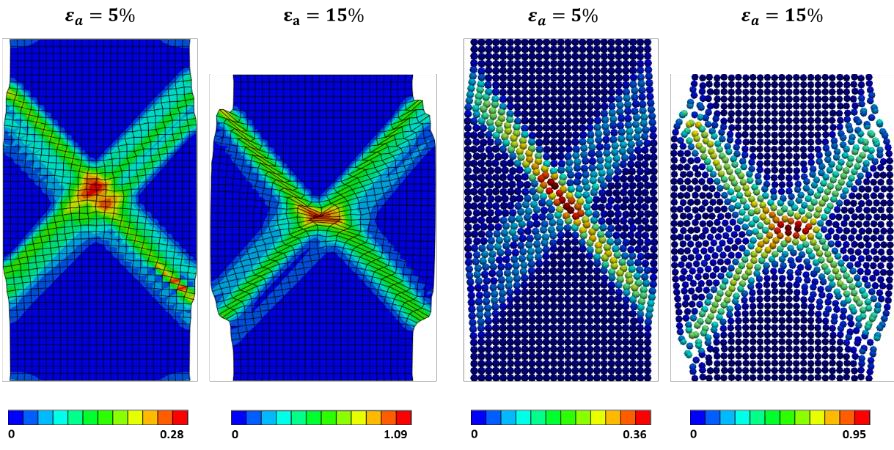
\includegraphics[width=0.95\textwidth]{5-11.png}
\caption{Biaxial test results from FEM (left) and SPH (right).}\label{fig:5}
\end{figure}

\end{abstract}


%%THE END OF ABSTRACT

\addbib

\end{document}
